% !TeX spellcheck = en_US
% !TeX root = notes.tex
\subsection{Link Layer}
\begin{itemize}
	\item hosts and routers: \textbf{nodes}
	\item communication channels that connect adjacent nodes along communication path: \textbf{links}
	\item layer-2 packet: \textbf{frame}, encapsulates datagram
\end{itemize}
\begin{note}{Link Layer Introduction}
	\textbf{data-link layer} has responsibility of transferring datagram from one node to \textbf{physically adjacent} node over a link
\end{note}
\subsubsection{Link layer services}
\begin{itemize}
	\item \textbf{framing, link access}
	\begin{itemize}
		\item encapsulate datagram into frame, adding header, trailer
		\item channel access if shared medium
		\item ``MAC'' addresses used in frame headers to identify source, destination (different from IP address!)
	\end{itemize}
	\item \textbf{reliable delivery between adjacent nodes}
	\begin{itemize}
		\item seldom used on low bit-error link (fiber, some twisted pair)
		\item wireless links: high error rates
	\end{itemize}
	\item \textbf{Flow Control:} pacing between adjacent sending and receiving nodes
	\item \textbf{error detection}
	\begin{itemize}
		\item errors caused by signal attenuation, noise
		\item receiver detects presence of errors: signals sender for retransmission or drops frame
	\end{itemize}
	\item \textbf{error correction:} receiver identifies \textbf{and corrects} bit error(s) without resorting to retransmission
	\item \textbf{half-duplex and full-duplex:} with half duplex, nodes at both ends of link can transmit, but not at same time
\end{itemize}
Link layer is implemented in the adapter (aka \textbf{network interface card (NIC)})

\subsection{Error Detection}
\subsubsection{Parity Checking}
\textbf{single bit parity:} detect single bit errors\\
\textbf{two-dimensional bit parity:} detect and correct single bit errors
\subsubsection{Cyclic Redundancy Check}
\begin{itemize}
	\item more powerful error-detection coding
	\item view data bits, $D$, as a binary number
	\item choose $r+1$ bit pattern (generator), $G$
	\item goal: choose $r$ CRC bits, $R$, such that
	\begin{itemize}
		\item $<D,R>$ exactly divisible by $G$ (modulo 2)
		\item receiver knows $G$, divides $<D,R>$ by $G$. If non-zero remainder: error detected!
		\item can detect all burst errors less than $r+1$ bits
	\end{itemize}
	\item widely used in practice (Ethernet, 802.11 WiFi, ATM)
\end{itemize}

\subsection{Multiple access links, protocols}
\begin{itemize}
	\item point-to-point
	\begin{itemize}
		\item PPP for dial-up access
		\item point-to-point link between Ethernet switch, host
	\end{itemize}
	\item broadcast (shared wire or medium)
	\begin{itemize}
		\item old-fashioned Ethernet
		\item upstream HFC
	\end{itemize}
\end{itemize}
\begin{note}{Multiple Access Protocol}
	\begin{itemize}
		\item distributed algorithm that determines how nodes share channel, i.e. determine when node can transmit
		\item communication about channel sharing must use channel iteself! (no out-of-band channel for coordination)
	\end{itemize}
\end{note}
Given a broadcast channel of rate $R$ bps. An ideal multiple access protocol needs:
\begin{itemize}
	\item when one node wants to transmit, it can send at rate $R$
	\item when $M$ nodes want to transmit, each can send at average rate $\frac{R}{M}$
	\item fully decentralized:
	\begin{itemize}
		\item no special node to coordinate transmissions
		\item no synchronization of clocks, slots
	\end{itemize}
	\item simple
\end{itemize}

\subsection{MAC Protocols}
\begin{description}
	\item[Channel Partitioning:] divide channel into smaller ``pieces'' (time slots, frequency, code). Allocate piece to node for exclusive use
	\item[Random Access:] channel not divided, allow collisions, ``recover'' from collisions
	\item[``Taking Turns'':] nodes take turns, but nodes with more to send can take longer turns
\end{description}
\subsubsection{TDMA: time division multiple access}\label{sec:tdma}
\begin{itemize}
	\item access to channel in ``rounds''
	\item each station gets fixed length slot (length = packet transmission time) in each round
	\item unused slots go idle
\end{itemize}
\subsubsection{FDMA: frequency division multiple access}\label{sec:fdma}
\begin{itemize}
	\item channel spectrum divided into frequency bands
	\item each station assigned fixed frequency band
	\item unused transmission time in frequency bands go idle
\end{itemize}

\subsection{Random Access Protocols}
\begin{itemize}
	\item when node has packet to send
	\begin{itemize}
		\item transmit at full channel data rate $R$
		\item no examination between nodes prior
	\end{itemize}
	\item two or more transmitting nodes $\rightarrow$ ``collision''
	\item \textbf{random access MAC protocol} specifies:
	\begin{itemize}
		\item how to detect collisions
		\item how to recover from collisions (e.g. via delayed retransmissions)
	\end{itemize}
	\item examples of random access MAC protocols:
	\begin{itemize}
		\item slotted ALOHA
		\item ALOHA
		\item CSMA, CSMA/CD, CSMA/CA
	\end{itemize}
\end{itemize}
\subsubsection{Slotted ALOHA}\label{sec:saloha}
\textbf{Assumptions:}
\begin{itemize}
	\item all frames same size
	\item time divided into equal size slots (time to transmit 1 frame)
	\item nodes start to transmit only slot beginning
	\item nodes are synchronized
	\item if 2 or more nodes transmit in slot, all nodes detect collision
\end{itemize}
\textbf{Operation:}
\begin{itemize}
	\item when node obtains fresh frame, transmits in next slot
	\begin{itemize}
		\item if no collision: node can send new frame in next slot
		\item if collision: node retransmits frame in each subsequent slot with probability $p$ until success
	\end{itemize}
\end{itemize}
\textbf{Pros:}
\begin{itemize}
	\item single active node can continuously transmit at full rate of channel
	\item highly decentralized: only slots in nodes need to be in sync
	\item simple
\end{itemize}
\textbf{Cons:}
\begin{itemize}
	\item collisions, wasting slots
	\item idle slots
	\item nodes may be able to detect collision in less than time to transmit packet
	\item clock synchronization
\end{itemize}
\subsubsection{Pure (unslotted) ALOHA}\label{sec:paloha}
\begin{itemize}
	\item unslotted Aloha: simpler, no synchronization
	\item when frame first arrives $\rightarrow$ transmit immediately
	\item collision probability increases: frame sent at $t_0$ collides with other frames sent in $[t_0-1,t_0+1]$
\end{itemize}
\subsubsection{CSMA (carrier sense multiple access)}\label{sec:CSMA}
\textbf{CSMA:} listen before transmit
\begin{itemize}
	\item \textbf{if channel sensed idle:} transmit entire frame
	\item \textbf{if channel sensed busy:} defer transmission
	\item \textbf{collisions can still occur:} propagation delay means two nodes may not hear each other's transmission
	\item \textbf{collision:} entire packet transmission time wasted (distance and propagation delay play role in determining collision probability)
\end{itemize}
\subsubsection{CSMA/CD (collision detection)}\label{sec:CSMA/CD}
\textbf{CSMA/CD:} carrier sensing, deferral as in CSMA
\begin{itemize}
	\item collisions \textit{detected} within short time
	\item colliding transmissions aborted, reducing channel wastage
	\item collision detection:
	\begin{itemize}
		\item easy in wired LANs: measure signal strengths, compare transmitted, received signals
		\item difficult in wireless LANs: received signal strength overwhelmed by local transmission strength
	\end{itemize}
\end{itemize}
\begin{enumerate}
	\item NIC receives datagram from network layer, create frame
	\item If NIC sense channel idle, starts frame transmission. If NIC sense channel busy, waits until channel idle, then transmits
	\item If NIC transmits entire frame without detecting another transmission, NIC is done with frame
	\item If NIC detects another transmission while transmitting, aborts and sends jam signal
	\item After aborting, NIC enter \textbf{binary (exponential) backoff:}
	\begin{itemize}
		\item after $m$th collision, NIC chooses $K$ at random from $\{ 0,1,2,\ldots,2^m-1 \}$. NIC waits $K\cdot512$ bit times, returns to Step 2
		\item longer backoff interval with more collisions
	\end{itemize}
\end{enumerate}
\begin{leftbar}
	Better performance than ALOHA
\end{leftbar}

\subsection{``Taking turns'' MAC protocols}
\textbf{Channel partitioning MAC protocols:}
\begin{itemize}
	\item share channel efficiently and fairly at high load
	\item inefficient at low load: delay in channel access, $\frac{1}{N}$ bandwidth allocated even if only 1 active node
\end{itemize}
\textbf{random access MAC protocols}
\begin{itemize}
	\item efficient at low load: single node can fully utilize channel
	\item high load: collision overhead
\end{itemize}
\textbf{``taking turns'' protocols:} look for best of both worlds!
\subsubsection{Polling}\label{sec:polling}
\begin{itemize}
	\item master node ``invites'' slave nodes to transmit in turn
	\item typically used with ``dumb'' slave devices
	\item concerns: polling overhead, latency, single point of failure (master)
\end{itemize}
\subsubsection{Token Passing}\label{sec:token}
\begin{itemize}
	\item control \textbf{token} passed from one node to next sequentially
	\item token message
	\item concerns: token overhead, latency, single point of failure (token)
\end{itemize}

\subsection{Cable Access Network}
\subsubsection{DOCSIS: Data Over Cable Service Interface Spec}\label{sec:docsis}
\begin{itemize}
	\item FDM over upstream, downstream frequency channels
	\item TDM upstream: some slots assigned, some have contention
	\begin{itemize}
		\item downstream MAP frame: assigns upstream slots
		\item request for upstream slots (and data) transmitted random access (binary backoff) in selected slots
	\end{itemize}
\end{itemize}

\subsection{MAC Addresses and ARP}
32-bit IP address:
\begin{itemize}
	\item network-layer address for interface
	\item used for layer 3 (network layer) forwarding
\end{itemize}
MAC (or LAN or physical or Ethernet) address:
\begin{itemize}
	\item function: used `locally' to get frame from one interface to another physically-connected interface (same network, in IP-addressing sense)
	\item 48 bit MAC address (for most LANs) burned in NIC ROM, also sometimes software settable
\end{itemize}
\subsubsection{LAN Address}
\begin{itemize}
	\item MAC address allocation administered by IEEE
	\item manufacturer buys portion of MAC address space (to assure uniqueness)
	\item MAC flat address $\rightarrow$ portability (can move LAN card from one LAN to another)
	\item IP hierarchical address not portable (address depends on IP subnet to which node is attached)
\end{itemize}
\subsubsection{ARP: Address Resolution Protocol}\label{sec:arp}
\textbf{ARP table:} each IP node (host, router) on LAN has table
\begin{itemize}
	\item IP/MAC address mappings for some LAN nodes: \texttt{<IP address; MAC address; TTL>}
	\item TTL (Time To Live): time after which address mapping will be forgotten (typically 20 mins)
\end{itemize}

\subsection{Ethernet}
\subsubsection{Physical Topology}
\begin{description}
	\item[bus:] popular through mid 90s (all nodes in same collision domain (can collide with each other))
	\item[star:] prevails today (active \textbf{switch} in center, each ``spoke'' runs a (separate) Ethernet protocol (nodes do not collide with each other))
\end{description}
\subsubsection{Ethernet frame structure}
\begin{table}[H]
	\centering
	\caption{Ethernet Frame Structure}
	\begin{tabular}{c|p{1cm}|p{1cm}|c|p{1cm}|c}
		7b & 6b & 6b &&&\\
		\midrule
		preamble & dest addr & source addr & type & data (payload) & CRC
	\end{tabular}
\end{table}
\begin{description}
	\item[preamble:] 7 bytes with pattern 10101010 followed by one byte with pattern 10101011. Used to synchronize receiver, sender clock rates
	\item[addresses:] 6 byte source, destination MAC addresses
	\begin{itemize}
		\item if adapter receives frame with matching destination address, or with broadcast address (e.g. ARP packet), it passes data in frame with network layer protocol
		\item otherwise, adapter discards frame
	\end{itemize}
	\item[type:] indicated higher layer protocol (mostly IP but others possible, e.g. Novell IPX, AppleTalk)
	\item[CRC:] cyclic redundancy check at receiver (error detected: frame is dropped)
\end{description}
\subsubsection{Ethernet: unreliable, connectionless}
\begin{description}
	\item[connectionless:] no handshaking between sending and receiving NICs
	\item[unreliable:] receiving NIC doesn't send acks or nacks to sending NIC (data in dropped frames recovered only if sender uses higher layer rdt (e.g. TCP), otherwise dropped data lost)
\end{description}
Ethernet's MAC protocol: unslotted \textbf{CSMA/CD with binary backoff}
\subsubsection{Ethernet switch}
\begin{description}
	\item[link-layer device:] takes an active role
	\begin{itemize}
		\item store, forward Ethernet frames
		\item examine incoming frame's MAC address, \textbf{selectively} forward frame to one-or-more outgoing links when frame is to be forwarded on segment, uses CSMA/CD to access segment
	\end{itemize}
	\item[transparent:] hosts are unaware of presence of switches
	\item[plug-and-play, self-learning:] switches do not need to be configured
\end{description}

\subsection{Switches vs routers}
both are store-and-forward:
\begin{description}
	\item[routers:] network-layer devices (examine network-layer headers)
	\item[switches:] link-layer devices (examine link-layer headers)
\end{description}
both have forwarding tables:
\begin{description}
	\item[routers:] compute tables using routing algorithms, IP addresses
	\item[switches:] learn forwarding table using flooding, learning, MAC addresses
\end{description}

\subsection{VLANs}
\begin{note}{Virtual Local Area Network}
	switch(es) supporting VLAN capabilities can be configured to defined multiple \textbf{virtual} LANs over single physical LAN infrastructure
\end{note}
\subsubsection{Port-based VLAN}
switch ports grouped (by switch management software) so that \textbf{single} physical switch operates as \textbf{multiple} virtual switches
\begin{description}
	\item[traffic isolation:] frames to/from ports 1-8 can \textit{only} reach ports 1-8 (can also define VLAN based on MAC addresses of endpoints, rather than switch port)
	\item[dynamic membership:] ports can be dynamically assigned among VLANs
	\item[forwarding between VLANs:] done via routing (just as with separate switches). In practice vendors sell combined switches plus routers
\end{description}
\textbf{VLANs spanning multiple switches}
\begin{description}
	\item[trunk port:] carries frames between VLANs defined over multiple physical switches
	\begin{itemize}
		\item frames forwarded within VLAN between switches can't be vanilla 802.1 frames (must carry VLAN ID info)
		\item 802.1q protocol adds/removed additional header fields for frames forwarded between trunk ports
	\end{itemize}
\end{description}
\begin{figure}[H]
	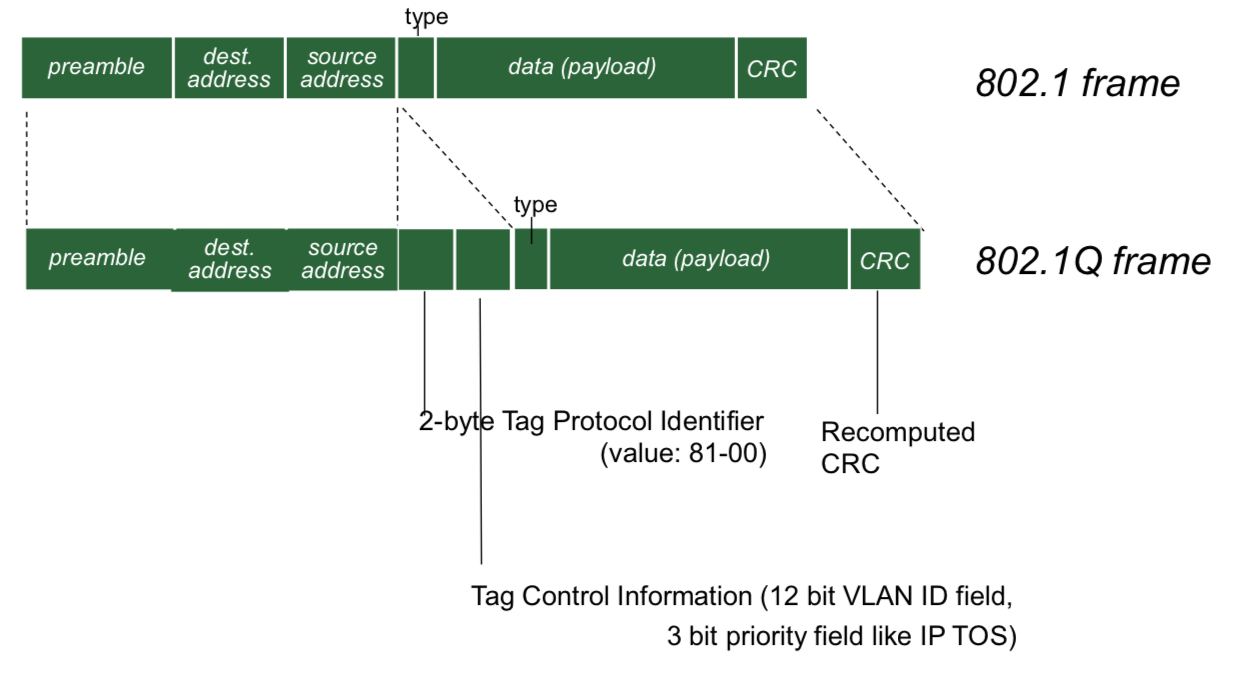
\includegraphics[width=\linewidth]{802q}
	\centering
	\caption{802.1Q VLAN frame format}
\end{figure}